\documentclass{standalone}
\usepackage{tikz}
\usetikzlibrary{decorations.pathmorphing,patterns}
\begin{document}
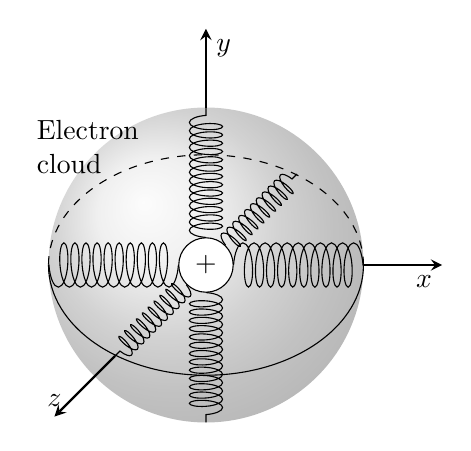
\begin{tikzpicture}
    
    % Ball + equator
    \shade[ball color = gray!40, opacity = 0.4] (0,0) circle (2);
    \draw (-2,0) arc (180:360:2 and 1.4);
    \draw[dashed] (2,0,0) arc (0:180:2 and 1.4);
    \draw node[draw,fill=white,circle]{+};
    
    % Axes
    \draw[thick,->, >=stealth] (2,0,0) -- (3,0,0) node[anchor=north east]{$x$};
    \draw[thick,->, >=stealth] (0,2,0) -- (0,3,0) node[anchor=north west]{$y$};
    \draw[thick,->, >=stealth] (0,0,3) -- (0,0,5) node[anchor=south]{$z$};
    
    % Diff springs
    \draw[decoration={aspect=0.3, segment length=4, amplitude=8, coil},decorate] 
    (0.35,0,0) -- (2,0,0);
    \draw[decoration={aspect=0.3, segment length=4, amplitude=8, coil},decorate] 
    (-0.35,0,0) -- (-2,0,0);
    
    \draw[decoration={aspect=0.3, segment length=3, amplitude=6, coil},decorate] 
    (0,0.35,0) -- (0,2,0);
    \draw[decoration={aspect=0.3, segment length=3, amplitude=6, coil},decorate] 
    (0,-0.35,0) -- (0,-2,0);
    
    \draw[decoration={aspect=0.3, segment length=3, amplitude=4, coil},decorate] 
    (0,0,0.65) -- (0,0,3);
    \draw[decoration={aspect=0.3, segment length=3, amplitude=4, coil},decorate] 
    (0,0,-0.65) -- (0,0,-3);
    
    % Text
    \node[align=left] at (-1.5,1.5,0) {Electron\\ cloud};
    
\end{tikzpicture}
\end{document}